\section{Conclusiones}
Después de las pruebas llevadas a cabo, podemos concluir el proyecto con un enfoque positivo. Gracias a la infraestructura de red creada, se ha conseguido con éxito una recopilación de datos colaborativa partiendo de un fichero inicial de datos desde el ordenador central, pasando por todos los nodos de la red y llegando, de nuevo, al ordenador central.

La información aportada por cada uno de los nodos de la red, está desligada de su dirección IP, de forma que, a priori, no se conozca la información que añadió cada nodo. El único inconveniente de esto es que, al ser una cadena secuencial, solo tendremos que saber qué nodos están conectados a la red para saber la información añadida por cada nodo.

Se pueden destacar varios escenarios de trabajo:
\begin{itemize}
	\item Si todos los nodos están conectados correctamente a la red, se producirá un recorrido lineal que partirá desde el ordenador central, viajará por todos los nodos desde zybo1 hasta zyboX. Una vez que se recorra toda la cadena y, al no detectar el siguiente nodo, zybo(X+1), el fichero retornará al ordenador central.
	\begin{figure}[h]
		\centering
		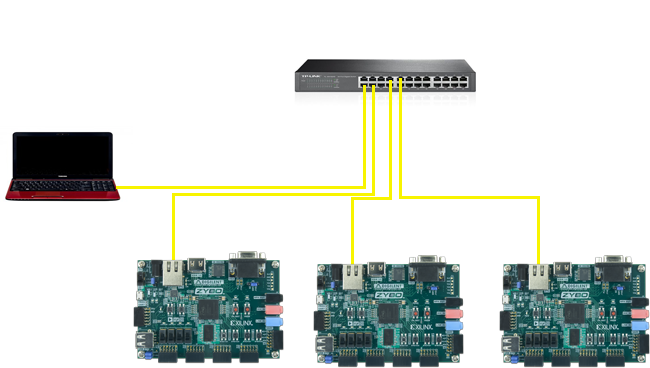
\includegraphics[scale=0.5]{Epilogo/RedCompleta.png}
		\caption{Red completa}
		\label{Red completa}
	\end{figure}
	\item Cuando algún nodo intermedio de la red está desconectado, la cadena se romperá y, el nodo anterior, al no conseguir comunicación, enviará el fichero con la información recopilada al ordenador central, obviando el resto de nodos.
	\begin{figure}[h]
		\centering
		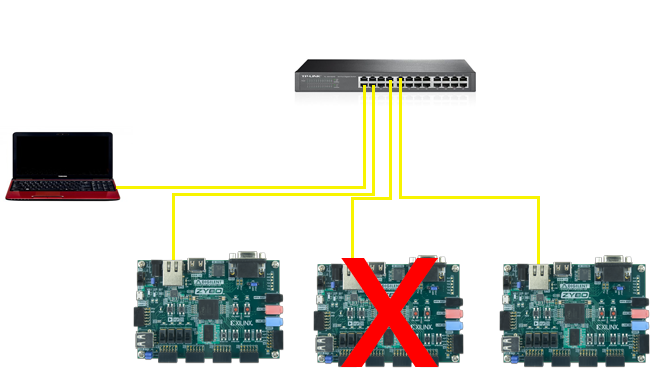
\includegraphics[scale=0.5]{Epilogo/RedSinNodo2.png}
		\caption{Red sin nodo intermedio}
		\label{Red sin nodo intermedio}
	\end{figure}
	\item Otro escenario será cuando el primer nodo de la red está desconectado.
	\begin{figure}[h]
		\centering
		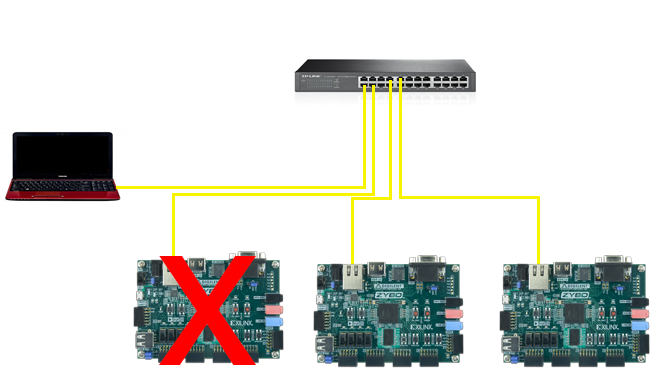
\includegraphics[scale=0.5]{Epilogo/RedSinNodo1.png}
		\caption{Red sin primer nodo}
		\label{Red sin primer nodo}
	\end{figure}\\
	Entonces, tendremos dos opciones:
	\begin{itemize}
		\item Volver a revisar la conexión con el primer nodo hasta conseguir solucionar el problema.
		\item Usar como primer nodo el segundo, enviando el fichero inicial directamente al segundo nodo de la red.
	\end{itemize}
\end{itemize}

\section{Trabajo futuro}
Como trabajo futuro quedaría cambiar la cadena de conexiones y que, en vez de recorrer los nodos de forma secuencial, se hiciera de forma aleatoria, para que no se supiera qué nodo ha seguido a cual. De esta forma, se conseguirá un desconocimiento total por parte del ordenador central sobre qué nodo añadió cada información al fichero final.

También se podría mejorar el proyecto incluyendo un módulo Wi-Fi, de modo que los nodos, no tengan que estar necesariamente conectados por cable. Esto nos daría la posibilidad de ubicar cada nodo donde quisiéramos (dentro de las capacidades físicas de la red Wi-Fi) y así poder usar dicha estructura en un entorno de IoT\footnote{Internet of Things.} para una casa o el edificio que necesitemos.

Este proyecto nos aporta una gran ventaja frente a la seguridad informática ya que, los ficheros transmitidos están doblemente cifrados, tanto por el propio protocolo SSH como por el IP cifrador/descifrador AES incorporado en los nodos Zybo. Esto hace que podamos recrearlo en cualquier red sin miedo a posibles filtraciones de datos.